\documentclass[pdftex,a4paper,12pt,twocolumn,fleqn,captions=tableheading]{scrartcl}

\usepackage[british]{babel}
\usepackage[utf8]{inputenc}
\usepackage[T1]{fontenc}
\usepackage{graphicx}
\usepackage{booktabs}
\usepackage{caption}
\usepackage{subcaption}
\usepackage{lmodern}
\usepackage{microtype}
\usepackage{textcomp}
\usepackage{amssymb}
\usepackage{epstopdf}
\usepackage{capt-of}
\usepackage{amsmath}
\usepackage{float}
\usepackage{xfrac}
\usepackage{dblfloatfix}
\usepackage{url}
\usepackage[squaren,Gray]{SIunits}
\usepackage{commath}
\usepackage{listings}
% \usepackage{siunitx}

\addtokomafont{caption}{\small}
\setkomafont{captionlabel}{\sffamily\bfseries}

\usepackage[nottoc]{tocbibind}

% page layout
\usepackage[a4paper,onecolumn]{geometry}
\geometry{hmargin=60pt,top=60pt,bottom=80pt}
% \geometry{onecolumn,columnsep=20pt}
\geometry{head=10pt,headsep=20pt,foot=35pt}

% header and footer
\usepackage{fancyhdr}
\setlength{\headheight}{15pt}
\pagestyle{fancy}
%\fancyheadoffset{9pt}
%\fancyfootoffset{9pt}
\lhead{}	\chead{User manual IMU loggers}	\rhead{}
\lfoot{}	\cfoot{J. Rabault \\ \thepage}	\rfoot{}
%\renewcommand{\headrulewidth}{0,1 mm}
\renewcommand{\footrulewidth}{\headrulewidth}

\begin{document}
% top matter
\title{Using the waves in ice IMU loggers}
\author{J. Rabault
  }
\date{\today}

\maketitle

\section{Introduction}

This document gives some details about how to use the IMU loggers. Each logger is equipped with an IMU, a GPS chip and antenna, a SD card and a microcontroller. There are two logger models: the yellow ones and the orange ones. The only difference is in the battery model and size and therefore the weigth of the loggers, while the underlying electronics are the same. The orange loggers are larger, heavier and have better battery capacity.

\section{Use}

It is best to switch the loggers on and off in the boat if possible, and to avoid opening the loggers when outside in order to limit the amount of water, snow and humidity in the loggers. If you recover the loggers and they are wet, first dry them before opening. The procedure for using the loggers is the following:

\begin{itemize}
  \item Make sure that the SD card is present in the SD card reader (see Fig. \ref{SDwithCard}).

  \begin{figure}
  \begin{center}
  \includegraphics[width=.4\textwidth]{Figures/IMG_20170418_134552}
  \caption{\label{SDwithCard} The SD card reader, with the inserted SD card (format mini). The SD card LED is active.}
  \end{center}
  \end{figure}

  \item Put the loggers on. For the yellow loggers, this means plugging the USB cable into the power bank (in one of the outputs, just avoid the 0.5A one that may be too weak), and pressing the button under the charge indication LEDs, see Fig. \ref{connectedYellow}. Once you press the button of the powerbank, power will be delivered to the logger. You can see the batter level by looking at the powerbank LEDs (1: 0 to 25 \%, 2: 25 to 50, 3: 50 to 75, 4: 75 to 100). For the orange loggers, simply connect the round connector of the battery to the round connector of the electronics, see Fig. \ref{connectedOrange}. The blue cable is not plugged when the logger is working (it is only used for cell balancing during charge).

  \begin{figure}
  \begin{center}
  \includegraphics[width=.8\textwidth]{Figures/IMG_20170418_102010}
  \caption{\label{connectedYellow} The yellow logger, connected, ready for logging.}
  \end{center}
  \end{figure}

  \begin{figure}
  \begin{center}
  \includegraphics[width=.8\textwidth]{Figures/IMG_20170418_102359}
  \caption{\label{connectedOrange} The orange logger, connected, ready for logging.}
  \end{center}
  \end{figure}

  \item Check that the logging is performed nominally. For this, you should look at the LEDs of the electronics board. There are three LEDs you could / should look at for ensuring that logging is performed properly. When first giving power to the logger, the ON LED of the arduino board should get green and stay on. This LED can be a bit difficult to see as it is under the hand-made board. This LED indicates that power is available for the logger. Then, the ACT and FIX LEDs, of the SD card board and the GPS card board respectively, should blink shortly. This indicates that the microncontroller is able to give current and talk to those boards. Finally, the GPS FIX LED should blink regularly with a period of about 1 second, while the SD card ACT LED should blink quickly, in an erratic manner. The frequency of the ACT LED should be several times per second, if it is slowly blinking or not blinking at all, see the troubleshooting section. For a view of the LEDs, see Figs. \ref{SDwithCard} and \ref{LEDsGPSArduino}

  \begin{figure}
  \begin{center}
  \includegraphics[width=.4\textwidth]{Figures/IMG_20170418_134534}
  \caption{\label{LEDsGPSArduino} Both the green LED of the board and the GPS LED are active.}
  \end{center}
  \end{figure}

  \item One you are sure that logging is performed nominally, make sure that all elements are securely disposed in the loggers (yellow loggers: electronics boards stable on the 3 pins, and powerbank stable in the foam with most cables stabilized under the powerbank; orange loggers: electronics board in the from slot, and stable foam; see Fig. \ref{readyClosing}). Then, close the pelicases. Be careful not to clamp cables when closing the pelicases. This can happen in particular with the cable to the GPS antenna. Clamping the cables can result in both cable damage and water infiltration.

  \begin{figure}
  \begin{center}
  \includegraphics[width=.45\textwidth]{Figures/IMG_20170418_134656}
  \includegraphics[width=.45\textwidth]{Figures/IMG_20170418_134711}
  \caption{\label{readyClosing} Loggers ready for closing the pelicases.}
  \end{center}
  \end{figure}

  \item To power off the loggers, simply cut the current supply. For the yellow loggers, press the power bank button and disconnect the USB on the power bank side. For the orange loggers, disconnect the cylindrical power connector. Note that data is written to a new file on the SD card every 15 minutes, and that the last file will be damaged during power shutoff. As a consequence, you should wait at least 15 minutes since the end of the interesting data being measured to power off the loggers, and if you perform a functionnality test less than 15 minutes long, you should not expect to have any data on the SD card.

\end{itemize}

\section{Deployment}

The are 3 yellow sensors, and 7 orange sensors. The yellow sensors only have an autonomy of about 24 hours when fully charged. The orange sensors have an autonomy of 8+ days when fully charged. The deployment guidelines for obtaining best data are the following:

\begin{itemize}
  \item If the floes are large enough, deploy the sensors by groups of 3, in a triangle configuration, each group of 3 sensors on the same floe. The sensors should be deployed at the angles of the triangle, and the distance between two sensors should be about 15 to 20 meters. Tie the three sensors together with a rope, to make recovery easier and keep the sensors grouped in case of floe dislocation. Make sure to measure accurately the distance between each pair of sensors, as the GPS accuracy is only typically a couple of meters but we need to rely on the distance between the sensors during processing. Also take note of the array orientation. See Fig. \ref{docEx3Sensors} for an example of technical documentation of an array deployment.

  \begin{figure}
  \begin{center}
  \includegraphics[width=.8\textwidth]{Figures/IMG_20170418_134237}
  \caption{\label{docEx3Sensors} Example of sensors deployment in an array of 3 format. In a real world situation, indicate the reference of each IMU sensor (the number, together with the letter in the case of the yellow sensor, on top of the pelicase).}
  \end{center}
  \end{figure}

  \item If the floes are too small for the triangle configuration, deploy the sensors individually, i.e. only one per small floe.

  \item If the boat stays close the the IMUs, no more precautions are needed. If the boat is to steam away from the sensors, attach one Iridium tracker to each individual or group of 3 sensors using a rope.

  \item The sensors float without the addition of any buoy, so using a buoy is not strictly needed. However, if you want to measure wave spectrum in the open water, use preferably the lighter yellow sensors (FX), together with a corresponding buoy. You can use the flags to make detection during recovery easier. A couple of heavier orange sensors can also be equipped with a buoy. You should use straps to fix the IMUs on the floats.

  \item GPS works best with a signal to the opened sky, try to avoid putting the loggers in an ice cavity or to bury them under more than a thin layer of snow.

  \item We are interested in several wave properties, in particular: wave spectrum, wave directional spectrum, and wave damping / wave spectrum evolution. Wave spectrum can be computed from one single sensor. Wave directional spectrum can be computed from either one single sensor or, better, from an array of 3 sensors in a triangle configuration. Wave damping / wave spectrum evolution can be computed by comparing the spectra and / or directional spectra obtained from distant sensors. Therefore, it is best to deploy groups of sensors (either 3 in a triangle configuration, or 1 on its own) as far away from each other, so that the clearest damping possible is visible. Several kilometers, if possible more, would be best.
\end{itemize}

\section{Data retrieval and parsing}

All data is logged on the mini SD card of each logger. As each logger keeps track of the last index used in the filemane for the data stored on its own SD card, it is important to always use the same SD card for the same logger. The procedure for retrieving the data is the following (should be performed for one logger after the other, in order to be sure not to mess up the SD cards):

\begin{itemize}
  \item Power off the logger, see the 'Use' section.

  \item Take out SD card. The SD card board has a 'press-in / out' system. Just press the SD card, and it should bounce back.

  \item Use SD card adapter (available together with the cables) to connect the SD card to a PC.

  \item Copy all files, one SD card content per folder. For ease of processing by scripts, follow the file tree given here. For example, if the date is 23/03/2017 and the SD card from the logger F1 contains files F00100, F00101 and F00102, create a folder 'Data\_IMU\_20032017' containing a folder 'F1', and in the folder F1 copy the files F00100, F00101 and F00102. If the logger 6 was also used, put all the data of the SD card corresponding to the logger 6 in a folder named '6', in parallel to the folder 'F1'. See Fig. \ref{folderstruct}. Some error messages can happen when copying files, because the last file used when power is switched off (which contains at most 15 minutes of data) gets corrupted. Those error messages can be ignored, and the corresponding files not copied.

  \begin{figure}
  \begin{center}
  \includegraphics[width=.4\textwidth]{Figures/IMG_20170418_135351}
  \caption{\label{folderstruct} Folder structure to use for easy data processing.}
  \end{center}
  \end{figure}

  \item When you are sure that the data has been copied, erase the SD card.

  \item Instert back the SD card, in the same logger as before. Insert it until you hear / feel a click.

  \item Make a copy of the whole data on a second data support to avoid data losses (i.e., external hard drive or another computer).

\end{itemize}

The data retrieved need to be parsed before further processing. If you need / want to look at the data, you can use the parser available here:

\begin{verbatim} https://github.com/jerabaul29/LoggerWavesInIce/tree/master/
          Logger_GPS_SD_VN_Binary_output_Parser \end{verbatim}
\end{verbatim}

\section{Charge}

All the battery cells use Lithium based battery. Be very careful when charing, bad charging could result in fire / explosion. Do not let the batteries unattended for long periods of time when charging.

The yellow loggers are equipped with one single power bank LiIon battery pack. The charging instructions for the yellow sensors are the following:

\begin{itemize}
  \item Turn off the power bank by pressing its side button.

  \item Disconnect the USB cable going into the power bank.

  \item Charge the power bank from either the USB port of a computer, or any USB charger (such as smartphone charger etc.). The port to use for charging is the 'input' mini USB. You may need to take the power bank completely out of the logger to perform charging.
\end{itemize}

The orange loggers are equipped with 2 LiFe cells, each giving around 3.2V at full charge and of capacity 40 Ah, assembled in series (2S). The special LiFe charger, with cells balancing, should be used. The charging instructions for the orange sensors are the following:

\begin{itemize}
  \item Disconnect the power connector of the logger.

  \item Assemble the charger, as shown in Fig. \ref{chargerAssembly}. Be very careful to make sure that you use the right polarity.

  \begin{figure}
  \begin{center}
  \includegraphics[width=.45\textwidth]{Figures/IMG_20170418_100240}
  \includegraphics[width=.45\textwidth]{Figures/IMG_20170418_100245}
  \caption{\label{chargerAssembly} Charger assembly: before and after.}
  \end{center}
  \end{figure}

  \item Make sure that the charger parameters are the correct ones: LiFe battery, and 3A charge. See Fig. \ref{chargerParams}.

  \begin{figure}
  \begin{center}
  \includegraphics[width=.8\textwidth]{Figures/IMG_20170418_100305}
  \caption{\label{chargerParams} Charge parameters are set using the charger switches.}
  \end{center}
  \end{figure}

  \item Plug both the cylindrical connector and the single wire into the battery pack. See Fig. \ref{ChargerPlugging}.

  \begin{figure}
  \begin{center}
  \includegraphics[width=.8\textwidth]{Figures/IMG_20170418_100414}
  \caption{\label{ChargerPlugging} Plug both the main power connector and the balance cable.}
  \end{center}
  \end{figure}

  \item Give AC 220V power to the chager. After a few seconds, the Charge status LED, and the 1S and 2S LEDs should turn red, see Fig \ref{InCharge}. If the battery cells are being balanced by the charger, it is possible that after some times just the 1S LED stays red while the 2S LED gets off.

  \begin{figure}
  \begin{center}
  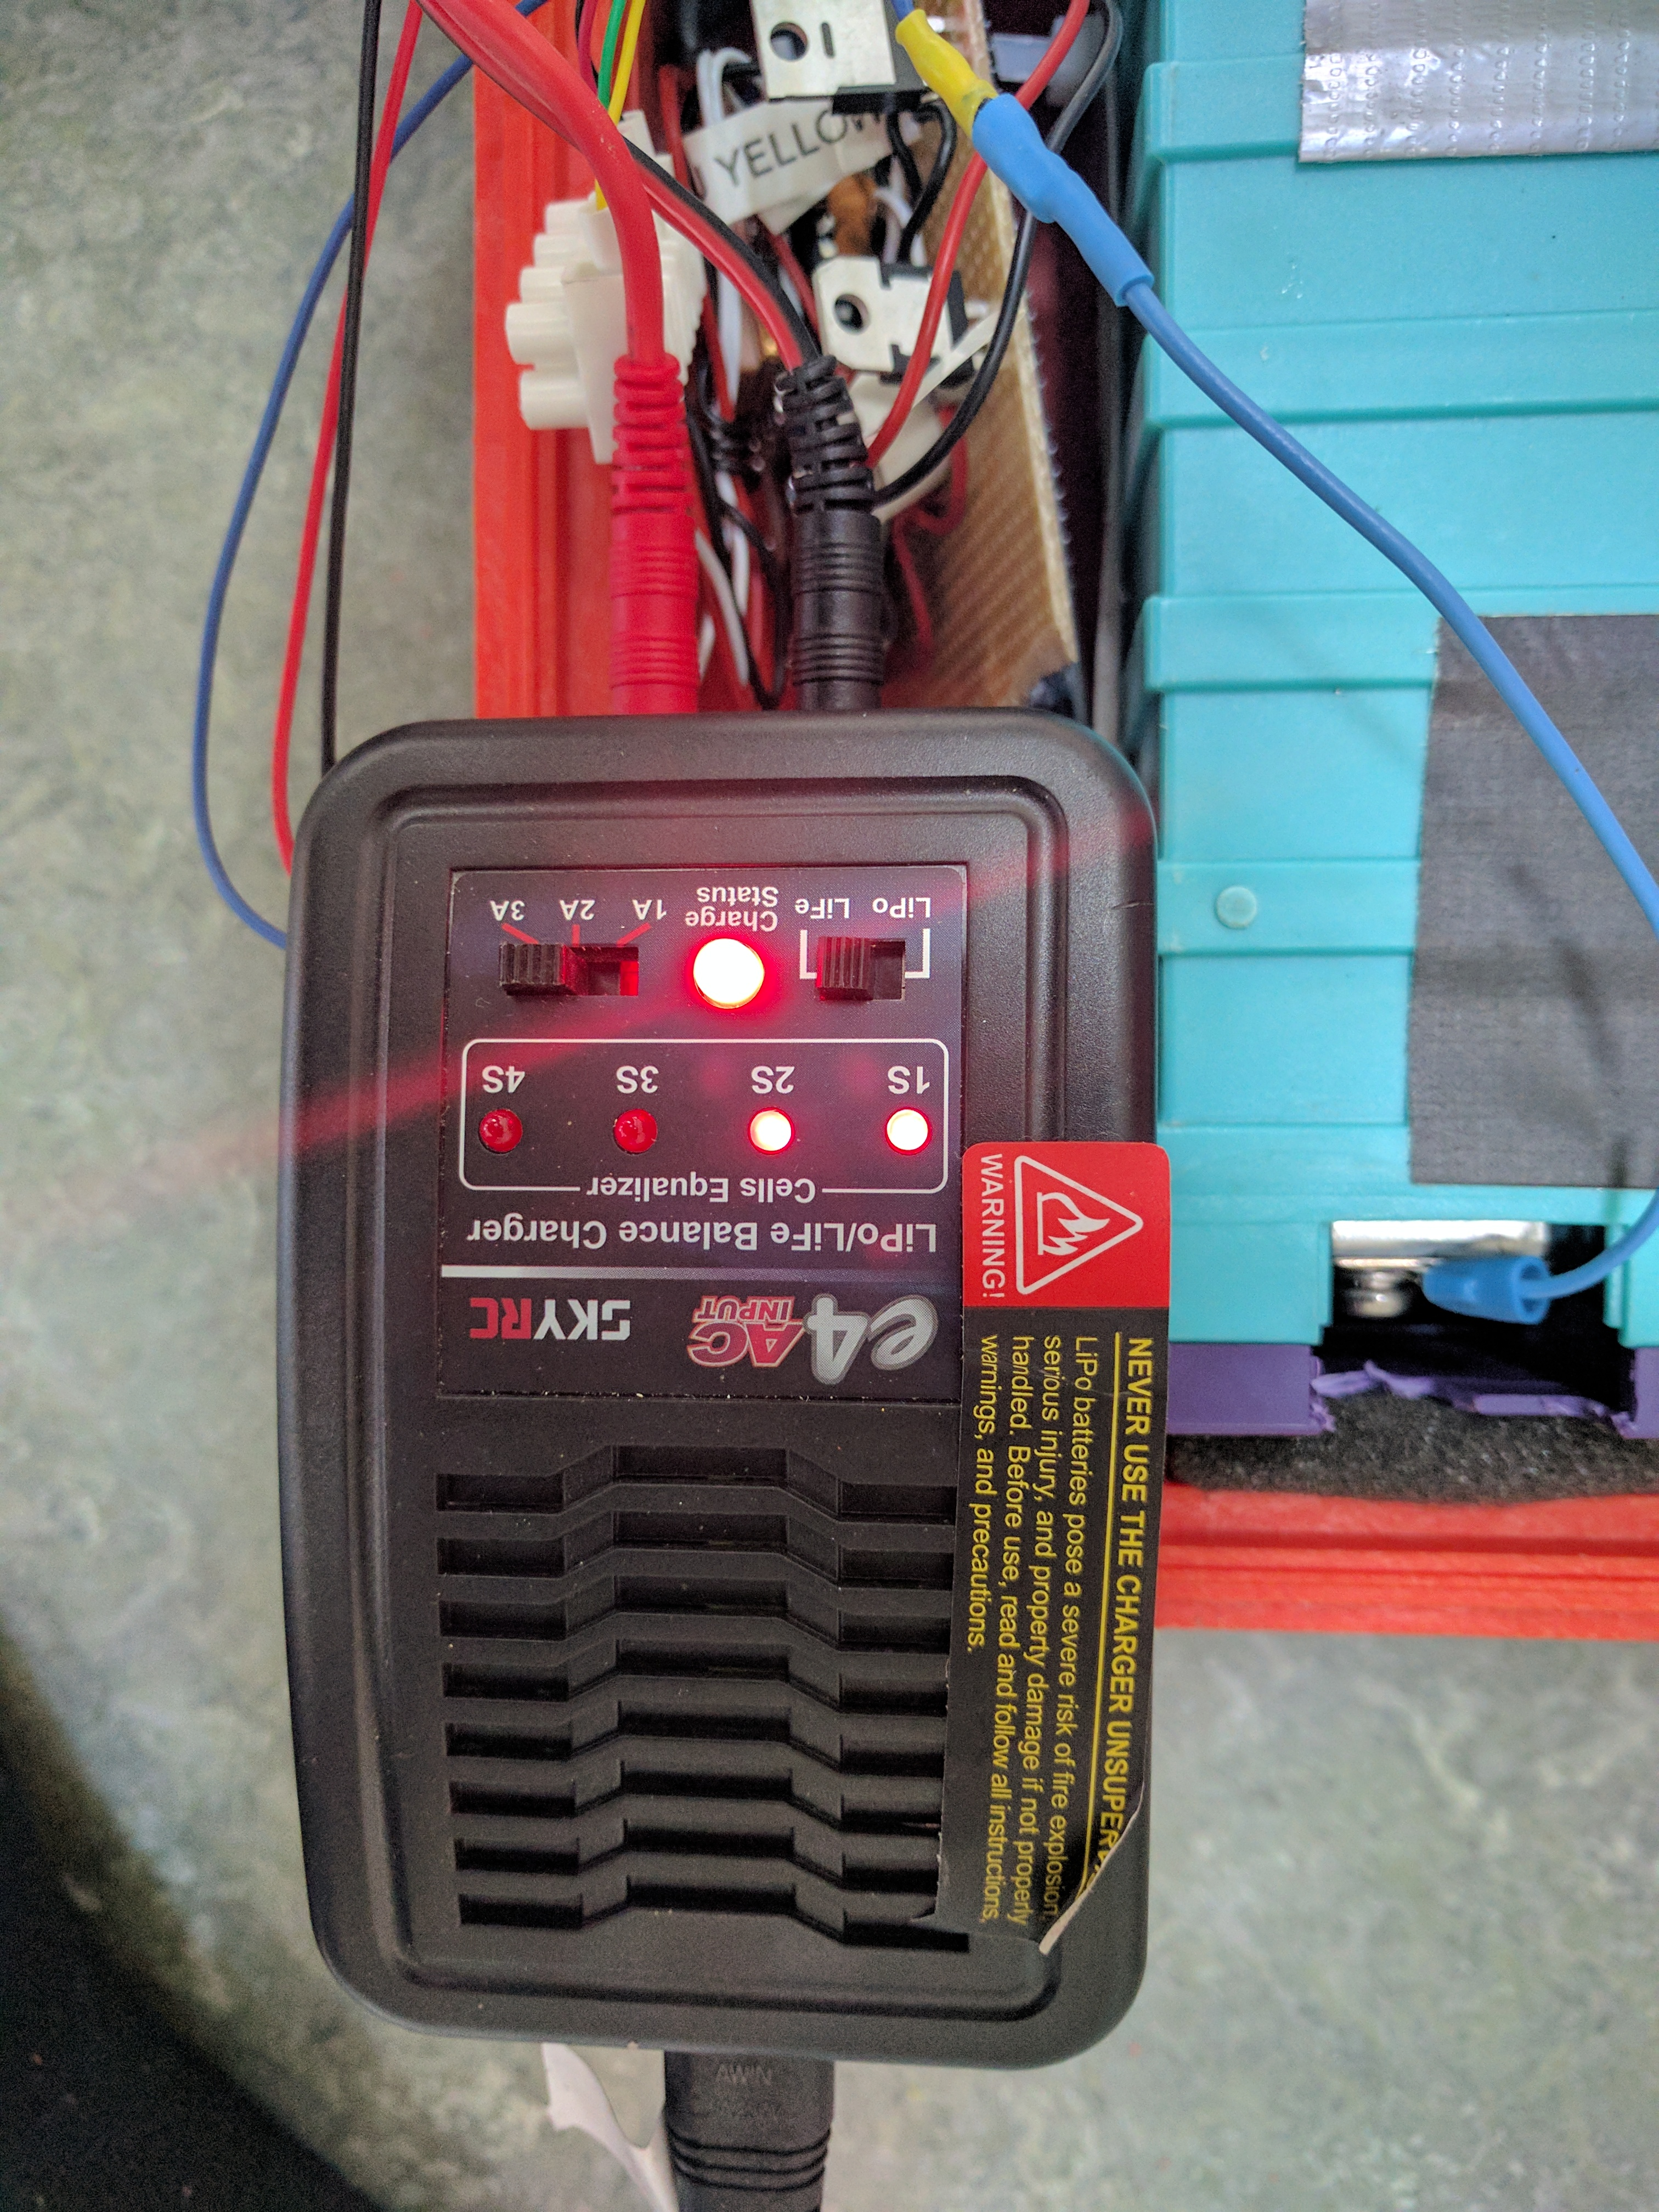
\includegraphics[width=.4\textwidth]{Figures/IMG_20170418_100127}
  \caption{\label{InCharge} Charging the 2S battery.}
  \end{center}
  \end{figure}

  \item When the Charge status LED turns green, the two cells are fully charged, see Fig \ref{Charged2S}. Note that, if the Charge status is green and blinking, this means that you forgot to connect the side cell balancing connector, but not that the cells are full.

  \begin{figure}
  \begin{center}
  \includegraphics[width=.4\textwidth]{Figures/IMG_20170418_102323}
  \caption{\label{Charged2S} Successfully charged 2S battery.}
  \end{center}
  \end{figure}

\end{itemize}

\section{Troubleshooting}

The loggers have been used in  3 measurements campaigns and always worked flawlessly. However a few minor issues were encounter due to rough handling of the loggers, such as large levels of vibration for a long transport on snow scooters, which can be easily fixed. Here is the list of the minor issues encountered so far, and how to fix them.

\begin{itemize}
  \item No light of the Arduino green LED: this may indicate depleted battery.

  \item No fast blinking of the SD card LED: make sure SD card correctly inserted (cause 1), check all electronics correctly inserted in each other (cause 2). Both cause 1 and 2 were observed after long, very bumpy snowscooter transport. Inserting back the boards into each other and plugging in and out the SD card solved the problem. It seems that the small connection board (see Fig. \ref{smallBoard}) especially has a tendency to bounce out under heavy vibration loads.

  \begin{figure}
  \begin{center}
  \includegraphics[width=.4\textwidth]{Figures/IMG_20170418_140411}
  \caption{\label{smallBoard} The small connection board can get disconnected under heavy sustained vibrations.}
  \end{center}
  \end{figure}

  \item The connectors to the GPS antenna (small gloden connector on the GPS board) easily get popped out or broken, be careful when handling the electronics. This may not be easily visible, but will degrade GPS signal quality.

\end{itemize}

If other issues occur, or you encounter any problem using or deploying the sensors: take contact with Jean Rabault: jean.rblt@gmail.com or jeanra@math.uio.no . In addition, fill in the log paper sheets attached in the faulty loggers describing the issue.

\end{document}
